\section{TỨ GIÁC NỘI TIẾP ĐƯỜNG TRÒN} % Tên bài
\subsection{TỨ GIÁC NỘI TIẾP ĐƯỜNG TRÒN}
\subsubsection{Chứng minh tứ giác nội tiếp}

\begin{tomtat}
\begin{boxdl}
	\begin{enumerate}
	\item \textbf{Chứng minh 4 điểm cách đều một đỉnh} 
	\immini{
		Nếu bốn đỉnh của một tứ giác cùng cách đều một điểm, thì bốn điểm đó cùng nằm trên một đường tròn. Do đó, tứ giác là tứ giác nội tiếp.\\
		Để tứ giác $ABCD$ nội tiếp được đường tròn thì phải chứng minh $OA=OB=OC=OD$.
	}{
		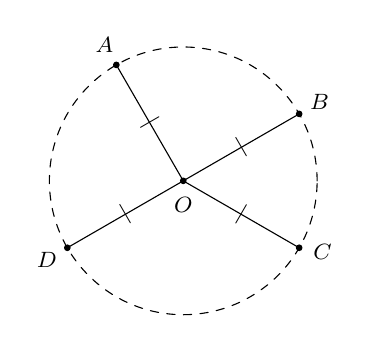
\begin{tikzpicture}[scale=1, font=\footnotesize, line join=round, line cap=round, >=stealth]
			\path
			(0,0)coordinate (O)
			(-30:1.7)coordinate (C)
			(210:1.7)coordinate (D)
			(120:1.7)coordinate (A)
			(30:1.7)coordinate (B)
			;
			\draw [dashed]
			(O) circle (1.7)	
			;
			\draw 
			(O)--(A)node[midway, sloped, rotate=0]{$|$}
			(O)--(B)node[midway, sloped, rotate=0]{$|$}
			(O)--(C)node[midway, sloped, rotate=0]{$|$}
			(O)--(D)node[midway, sloped, rotate=0]{$|$}
			;
			
			\foreach \x/\g in {A/120,B/30,C/-10,D/210,O/-90}\draw[fill=black] (\x) circle(1pt)+(\g:3mm) node {$\x$};
		\end{tikzpicture}
	}
	\textbf{Tính chất đường trung tuyến trong tam giác vuông:} Trong một tam giác vuông, đường trung tuyến ứng với cạnh huyền bằng một nửa cạnh huyền.
	\immini{
		Xét $\triangle ABC$ vuông tại $A$ có $AM$ là đường trung tuyến ứng với cạnh huyền $BC$ do đó
		$$ AM = BM = CM = \dfrac{1}{2}BC. $$
	}{
		\begin{tikzpicture}[scale=1, font=\footnotesize, line join=round, line cap=round, >=stealth]
			\path
			(0,0) coordinate (M)
			($(M)+(120:1.7)$) coordinate (A)
			($(M)+(180:1.7)$) coordinate (B)
			($(M)+(0:1.7)$) coordinate (C)
			;
			\draw 
			(M)--(A)node[midway, sloped, rotate=0]{$|$}
			(M)--(B)node[midway, sloped, rotate=0]{$|$}
			(M)--(C)node[midway, sloped, rotate=0]{$|$}
			(B)--(A)--(C)
			;
			\foreach \x/\g in {A/90,B/-90,C/-90,M/-90}\draw[fill=black] (\x) circle(1pt)+(\g:3mm) node {$\x$};
			\draw pic[draw,angle radius=2mm]{right angle=B--A--C};
		\end{tikzpicture}
	}
	\item \textbf{Chứng minh 4 điểm cùng thuộc một đường tròn}
	\immini{
		Đường tròn ngoại tiếp tam giác vuông có tâm là trung điểm của cạnh huyền và bán kính bằng nửa cạnh huyền của tam giác vuông đó.\\
		Xét $\triangle ABC$ vuông tại $A$, khi đó $\triangle ABC$ nội tiếp đường tròn đường kính $BC$.\\
		Suy ra $A$, $B$, $C$ cùng thuộc đường tròn đường kính $BC$. 
	}{
		\begin{tikzpicture}[scale=1, font=\footnotesize, line join=round, line cap=round, >=stealth]
			\path
			(0,0) coordinate (M)
			($(M)+(120:1.7)$) coordinate (A)
			($(M)+(180:1.7)$) coordinate (B)
			($(M)+(0:1.7)$) coordinate (C)
			;
			\draw 
			(B)--(A)--(C)--cycle
			;
			\draw[dashed] (M) circle(1.7);
			\foreach \x/\g in {A/90,B/180,C/0}\draw[fill=black] (\x) circle(1pt)+(\g:3mm) node {$\x$};
			\draw pic[draw,angle radius=2mm]{right angle=B--A--C};
		\end{tikzpicture}
	}
	\item \textbf{Chứng minh tứ giác nội tiếp thông qua chứng minh 5 điểm cùng thuộc một đường tròn}
\end{enumerate}
\end{boxdl}
\end{tomtat}

\begin{luuy}
	Hai mô hình thường gặp khi chứng minh tứ giác nội tiếp
	\begin{center}
		\begin{tikzpicture}[scale=1, font=\footnotesize, line join=round, line cap=round, >=stealth]
			\path
			(0,0) coordinate (O)
			($(O)+(120:1.7)$) coordinate (A)
			($(O)+(180:1.7)$) coordinate (B)
			($(O)+(0:1.7)$) coordinate (C)
			($(O)+(50:1.7)$) coordinate (D)
			;
			\draw
			(A)--(B)--(C)--(D)--(B) (C)--(A);
			;
			\foreach \x/\g in {A/90,B/-90,C/-90,D/90}\draw[fill=black] (\x) circle(1pt)+(\g:3mm) node {$\x$};
			\draw pic[draw,angle radius=2mm]{right angle=B--A--C};
			\draw pic[draw,angle radius=2mm]{right angle=B--D--C};
			\fill (0,2.7) node[below]{Mô hình 1};
			\begin{scope}[shift=({6,0})]
				\path
				(0,0) coordinate (O)
				($(O)+(120:1.7)$) coordinate (A)
				($(O)+(180:1.7)$) coordinate (B)
				($(O)+(0:1.7)$) coordinate (C)
				($(O)+(-100:1.7)$) coordinate (D)
				;
				\draw
				(A)--(B)--(C)--(D)--(B) (C)--(A);
				;
				\foreach \x/\g in {A/90,B/180,C/0,D/-90}\draw[fill=black] (\x) circle(1pt)+(\g:3mm) node {$\x$};
				\draw pic[draw,angle radius=2mm]{right angle=B--A--C};
				\draw pic[draw,angle radius=2mm]{right angle=B--D--C};
				\fill (0,2.7) node[below]{Mô hình 2};
			\end{scope}
		\end{tikzpicture}
	\end{center}
\end{luuy}

\begin{vd}%[Dự án EX-9-Đề Cương Toán 9]%[Lê Hòa Nam]%[9H3H2-1]
	Cho tam giác $ABC$ có ba góc nhọn. Vẽ các đường cao $BD$ và $CE$ của tam giác $ABC$. Gọi $H$ là giao điểm của $BD$ và $CE$.
	\begin{enumerate}
		\item Chứng minh $ADHE$ là tứ giác nội tiếp và xác định tâm của đường tròn đó.
		\item Chứng minh $BEDC$ là tứ giác nội tiếp và xác định tâm của đường tròn đó.
	\end{enumerate} 
	\loigiai{
		\begin{center}
			\begin{tikzpicture}[scale=1.2, font=\footnotesize, line join=round, line cap=round, >=stealth]
				
				\path
				(0,0)coordinate (B)
				(4,0)coordinate (C)
				(1.5,4)coordinate (A)
				($(C)!(B)!(A)$)coordinate (D)
				($(B)!(C)!(A)$)coordinate (E)
				;
				%Tìm giao điểm
				\draw[name path=aa] (C) -- (E);
				\draw[name path=bb] (B) -- (D);
				% Tìm giao điểm, đặt tên là B
				\path[name intersections={of=aa and bb, by=H}];
				
				%Giao điểm 2 đường
				%\path (intersection of D--E and C--B) coordinate (P);
				\path 
				($(B)!.5!(C)$)coordinate (J)
				($(A)!.5!(H)$)coordinate (I)
				;
				
				\draw 
				(A)--(B)--(C)--(A)
				(B)--(D) (C)--(E)
				;
				\draw (J) circle (2);
				
				\draw (I) circle (1.53);
				
				\draw
				pic[draw,angle radius=2mm]{right angle = B--D--C}
				pic[draw,angle radius=2mm]{right angle = B--E--C}
				(A)--(H)
				(J)--(B)node[midway, sloped, rotate=0]{$|$}
				(J)--(C)node[midway, sloped, rotate=0]{$|$}
				(I)--(A)node[midway, sloped, rotate=0]{$||$}
				(I)--(H)node[midway, sloped, rotate=0]{$||$}
				;
				\draw [dashed]
				(J)--(E)node[midway, sloped, rotate=0]{$|$}
				(J)--(D)node[midway, sloped, rotate=0]{$|$}
				(I)--(D)node[midway, sloped, rotate=0]{$||$}
				(I)--(E)node[midway, sloped, rotate=0]{$||$}
				;
				\foreach \x/\g in {A/90,B/180,C/0,D/30,E/180,H/-65,J/-90,I/20}\draw[fill=black] (\x) circle(1pt)+(\g:3mm) node {$\x$};
			\end{tikzpicture}
		\end{center}
		\begin{enumerate}
			\item Gọi $I$ là trung điểm $AH$.\\
			Xét $\triangle ADH$ vuông tại $D$, có $DI$ là đường trung tuyến ứng với cạnh huyền $AH$ nên
			$$DI = IA = IH = \dfrac{1}{2}AH. \qquad (1)$$
			Xét $\triangle AEH$ vuông tại $E$, có $EI$ là đường trung tuyến ứng với cạnh huyền $AH$ nên
			$$EI = IA = IH = \dfrac{1}{2}AH. \qquad (2)$$
			Từ $(1)$ và $(2)$ suy ra $EI = DI = IA = IH$ do đó bốn điểm $A$, $D$, $H$, $E$ cùng thuộc đường tròn tâm $I$ đường kính $AH$.\\
			Vậy tứ giác $ADHE$ nội tiếp đường tròn tâm $I$ đường kính $AH$.
			\item Gọi $J$ là trung điểm $BC$.\\
			Xét $\triangle BEC$ vuông tại $E$, có $EJ$ là đường trung tuyến ứng với cạnh huyền $BC$ nên
			$$EJ = JB = JC = \dfrac{1}{2}BC. \qquad (3)$$
			Xét $\triangle BDC$ vuông tại $D$, có $DJ$ là đường trung tuyến ứng với cạnh huyền $BC$ nên
			$$DJ = JB = JC = \dfrac{1}{2}BC. \qquad (4)$$
			Từ $(3)$ và $(4)$ suy ra $EJ = DJ = JB = JC$ do đó bốn điểm $B$, $E$, $D$, $C$ cùng thuộc đường tròn tâm $J$ đường kính $BC$.\\
			Vậy tứ giác $BEDC$ nội tiếp đường tròn tâm $J$ đường kính $BC$.
		\end{enumerate}
	}
\end{vd}

\subsubsection{Bài tập}

\begin{bt}%[Dự án EX-9-Đề Cương Toán 9]%[Lê Hòa Nam]%[9H3H2-1]
	Từ điểm $M$ nằm ngoài đường tròn $(O)$, vẽ cát tuyến $MBC$ và lần lượt các tiếp tuyến $MA$, $MD$ tiếp xúc với $(O)$ tại $A$, $D$ ($MC$ nằm trong $\widehat{DMO}$). Gọi $I$ là trung điểm của dây $BC$.
	\begin{enumerate}
		\item Chứng minh $AMIO$ là tứ giác nội tiếp.
		\item Chứng minh $DIOA$ là tứ giác nội tiếp.
	\end{enumerate}
	\loigiai{
		\begin{center}
			\begin{tikzpicture}[scale=0.9, line join=round, line cap=round,>=stealth, font=\footnotesize]
				\path
				(0,0)coordinate (O)
				(-8,0)coordinate (M)
				(-1.13,2.78)coordinate (A)
				(-1.13,-2.78)coordinate (D)
				(-2.85,-0.95)coordinate (B)
				(2.32,-1.9)coordinate (C)
				($(B)!.5!(C)$)coordinate (I)
				($(M)!.5!(O)$)coordinate (N)
				;
				\draw 
				(O)circle(3)
				(M)--(A)
				(M)--(D)
				(M)--(O)
				(M)--(C)
				(A)--(O)--(I) (N)--(A) (I)--(N)--(D)
				pic[draw,angle radius=2mm]{right angle = O--A--M}
				pic[draw,angle radius=2mm]{right angle = C--I--O}
				(I)--(D)--(A) (O)--(D)
				pic[draw,angle radius=2mm]{right angle = O--D--M}
				(B)--(O)--(C) 
				;
				\foreach \x/\g in {A/90,B/-135,C/-30,D/-90,M/180,O/30,I/-90,N/90}\draw[fill=black] (\x) circle(1pt)+(\g:3mm) node {$\x$};
			\end{tikzpicture}
		\end{center}
		\begin{enumerate}
			\item Xét tam giác $BOC$, có $OB=OC$ $(=R)$ nên tam giác $BOC$ cân, mà có $OI$ là đường trung tuyến suy ra $OI$ là đường cao hay $OI\perp BC$.\\
			Gọi $N$ là trung điểm của $MO$.\\
			Xét tam giác $AMO$ vuông tại $A$, có $AN$ là đường trung tuyến ứng với cạnh huyền $MO$ nên
			$$AN=NM=ND=\dfrac{1}{2}MO.\qquad (1)$$
			Xét tam giác $IMO$ vuông tại $I$, có $IN$ là đường trung tuyến ứng với cạnh huyền $MO$ nên
			$$IN=NM=NO=\dfrac{1}{2}MO.\qquad (2)$$
			Từ $(1)$ và $(2)$ suy ra $AN=IN=NM=NO$ do đó bốn điểm $A$, $M$, $D$, $O$ cùng thuộc đường tròn đường kính $MO$.\\
			Vậy tứ giác $AMIO$ nội tiếp đường tròn đường kính $MO$.
			\item Xét tam giác $DMO$ vuông tại $D$, có $DN$ là đường trung tuyến ứng với cạnh huyền $MO$ nên
			$$DN=NM=NO=\dfrac{1}{2}MO.\qquad (3)$$
			Từ $(1)$, $(2)$ và $(3)$ suy ra $AN=IN=DN=NM=NO$ do đó $5$ điểm $A$, $M$, $D$, $I$, $O$ cùng thuộc đường tròn đường kính $MO$.\\
			Vậy tứ giác $DIOA$ nội tiếp đường tròn đường kính $MO$.
		\end{enumerate}
	}
\end{bt}

\begin{bt}%[Dự án EX-9-Đề Cương Toán 9]%[Lê Hòa Nam]%[9H3V2-1]
	Cho đoạn thẳng $MP$, lấy điểm $N$ bất kì nằm giữa $M$ và $P$. Vẽ $(O)$ đường kính $NP$. Lấy $H$ là trung điểm của $MN$. Qua $H$ kẻ đường thẳng $d$ vuông góc với $MN$. Kẻ tiếp tuyến $HQ$ với $(O)$ tại $Q$. Tia $PQ$ cắt $d$ tại $K$. 
	\begin{enumerate}
		\item Chứng minh tứ giác $KHNQ$ nội tiếp và $\widehat{NPQ}=\widehat{HKN}$.
		\item Chứng minh $\widehat{MKP}=90^\circ$ và $PQ\cdot PK = PN\cdot PH$.
	\end{enumerate}
	\loigiai{
		\begin{center}
			\begin{tikzpicture}[scale=1, line join=round, line cap=round,>=stealth, font=\footnotesize]
				\path
				(-5,0)coordinate (M)
				(5,0)coordinate (P)
				(-1,0)coordinate (N)
				(2,0)coordinate (O)
				(-3,0)coordinate (H)
				(0.2,2.4)coordinate (Q)
				(-3,4)coordinate (K)
				;
				\draw 
				(O) circle (3)
				(M)--(P)
			(H)--(Q)
			(M)--(H)--(K)--(P)
			(M)--(K)--(N)--(Q)--(O)
			pic[draw,angle radius=2mm]{right angle = P--Q--N}
			pic[draw,angle radius=2mm]{right angle = K--H--N}
			pic[draw,angle radius=2mm]{right angle = M--K--P}
			pic[draw,angle radius=3mm]{right angle = O--Q--H}
				;
				\foreach \x/\g in {M/-90,H/-90,O/-90,P/0,K/180,Q/90,N/240}\draw[fill=black] (\x) circle(1pt)+(\g:3mm) node {$\x$};
			\end{tikzpicture}
		\end{center}
		\begin{enumerate}
			\item Xét tam giác $NQP$ nội tiếp đường tròn tâm $(O)$, có $\widehat{NQP}$ chắn cung $NP$ mà $NP$ là đường kính nên $\widehat{NQP}=90^\circ$.\\
			Gọi $I$ là trung điểm của cạnh $KN$.\\
			Xét tam giác vuông $QKN$ vuông tại $Q$, có $QI$ là đường trung tuyến ứng với cạnh huyền $KN$ nên
			$$QI=IK=IN=\dfrac{1}{2}KN. \qquad (1)$$
			Xét tam giác $HKN$ vuông tại $H$, có $HI$ là đường trung tuyến ứng với cạnh huyền $KN$ nên
			$$HI=IK=IN=\dfrac{1}{2}KN. \qquad (2)$$
			Từ $(1)$ và $(2)$, suy ra $QI=HI=IK=IN$ do đó bốn điểm $K$, $H$, $N$, $Q$ cùng thuộc đường tròn đường kính $KN$.\\
			Suy ra $KHNQ$ nội tiếp đường tròn tâm đường kính $KN$.\\
			Vì $HQ$ là tiếp tuyến của $(O)$ nên $\widehat{HQO}=90^\circ$ và $\widehat{NQP}=90^\circ$, suy ra $\widehat{HQN}=\widehat{OQP}$ (cùng phụ góc $\widehat{NQO}$).\\
			Mà $\widehat{OQP}=\widehat{OPQ}$ ($\triangle QOP$ cân tại $O$) nên $\widehat{OPQ}=\widehat{HQN}$ hay $\widehat{NPQ}=\widehat{HQN}$ $(3)$.\\
			Vì tứ giác $KHNQ$ nội tiếp nên $\widehat{HKN}=\widehat{HQN}$ (cùng chắn cung $HN$) $(4)$. \\
			Từ $(3)$ và $(4)$ suy ra $\widehat{NPQ}=\widehat{HKN}$.
			\item Vì $K$ nằm trên đường trung trực của đoạn $MN$ nên $KM=KN$ do đó tam giác $MKN$ cân tại $K$.\\
			Mà $KH$ là đường cao nên cũng $KH$ cũng là đường phân giác do đó $\widehat{MKH} = \widehat{HKN}$.\\
			Ta có
			\begin{itemize}
				\item $\widehat{MKH} = \widehat{HKN}$ (cmt),
				\item $\widehat{HKN}=\widehat{NPQ}$ (cmt),
				\item $\widehat{NPQ} + \widehat{HKN} = 90^\circ$.
			\end{itemize}
			Suy ra $\widehat{MKP} = \widehat{MKH} + \widehat{HKN} = 90^\circ$.\\
			Xét $\triangle PQN$ và $\triangle PHK$, ta có 
			\begin{itemize}
				\item $\widehat{HPK}$ chung,
				\item $\widehat{PQN} = \widehat{PHK}$ $(=90^\circ)$.
			\end{itemize}
			Suy ra $\triangle PQN\backsim\triangle PHK$ (g.g).\\ 
			Do đó $\dfrac{PQ}{PH} = \dfrac{PN}{PK}$ hay $PQ\cdot PK = PN\cdot PH$ (đpcm).
		\end{enumerate}
	}
\end{bt}

\begin{bt}%[Dự án EX-9-Đề Cương Toán 9]%[Lê Hòa Nam]%[9H3V2-1]
	Cho đường tròn $(O;R)$ và điểm $A$ nằm ở bên ngoài đường tròn. Vẽ hai tiếp tuyến $AB$, $AC$ với đường tròn $(O)$ ($B$, $C$ là các tiếp điểm). Gọi $M$ là trung điểm $AB$.
	\begin{enumerate}
		\item Chứng minh tứ giác $ABOC$ nội tiếp và xác định tâm $I$ của đường tròn.
		\item Chứng minh $AM\cdot AO = AB\cdot AI$.
		\item Gọi $G$ là trọng tâm tam giác $ACM$. Chứng minh $MG\parallel BC$.
	\end{enumerate}
	\loigiai{
	\begin{center}
		\begin{tikzpicture}[scale=1, line join=round, line cap=round,>=stealth, font=\footnotesize]
			\path
			(0,0)coordinate (O)
			(-7,0)coordinate (A)
			(-1.29,2.71)coordinate (B)
			(-1.29,-2.71)coordinate (C)
			($(A)!.5!(B)$)coordinate (M)
			($(A)!.5!(O)$)coordinate (I)
			($(A)!.5!(M)$)coordinate (E)
			($(C)!2/3!(E)$)coordinate (G)
			;
			
			\draw 
			(A)--(B)--(O)--(C)--(A) (O)--(A) (B)--(C) (M)--(I) (C)--(E) (G)--(M)--(C) 
			(O) circle (3)
			pic[draw,angle radius=2mm]{right angle = O--B--A}
			pic[draw,angle radius=2mm]{right angle = O--C--A}
			pic[draw,angle radius=2mm]{right angle = A--M--I}
			;
			\foreach \x/\g in {A/180,B/90,C/-90,O/0,M/90,I/-90,G/220,E/90}\draw[fill=black] (\x) circle(1pt)+(\g:3mm) node {$\x$};
		\end{tikzpicture}
	\end{center}
	\begin{enumerate}
		\item Gọi $I$ là trung điểm $AO$.\\
		Xét tam giác $ABO$ vuông tại $B$, có $BI$ là đường trung tuyến ứng với cạnh huyền $AO$ nên
		$$BI=IA=IO=\dfrac{1}{2}AO. \qquad (1)$$
		Xét tam giác $ACO$ vuông tại $C$, có $CI$ là đường trung tuyến ứng với cạnh huyền $AO$ nên
		$$CI=IA=IO=\dfrac{1}{2}AO. \qquad (2)$$
		Từ $(1)$ và $(2)$, suy ra $BI=CI=IA=IO$ do đó bốn điểm $A$, $B$, $O$, $C$ cùng thuộc đường tròn đường kính $AO$.\\
		Vậy tứ giác $ABOC$ nội tiếp đường tròn đường kính $AO$, có tâm $I$ là trung điểm $AO$.
		\item Ta có 
		\begin{itemize}
			\item $AM = \dfrac{1}{2}AB$ ($M$ là trung điểm của $AB$).
			\item $AO = 2AI$ ($I$ là trung điểm của $AO$).
		\end{itemize}
		Suy ra $AM\cdot AO = \dfrac{1}{2}AB\cdot 2AI = AB\cdot AI$ (đpcm).
		\item Gọi $E$ là trung điểm của $AM$.\\
		Xét tam giác $EBC$, có
		\begin{itemize}
			\item $EG=\dfrac{1}{3}EC$ ($G$ là trọng tâm) suy ra $\dfrac{EG}{EC} = \dfrac{1}{3}$.
			\item $EM=\dfrac{1}{3}EB$ ($M$ là trung điểm $AB$ và $E$ là trung điểm $AM$) suy ra $\dfrac{EM}{EB} = \dfrac{1}{3}$.
		\end{itemize}
		 Suy ra $\dfrac{EG}{EC}=\dfrac{EM}{EB}$ do đó $MG\parallel BC$ (định lý Thalès đảo).
	\end{enumerate}
	}
\end{bt}

\begin{bt}%[Dự án EX-9-Đề Cương Toán 9]%[Lê Hòa Nam]%[9H3C2-1]
	Cho đường tròn $(O;R)$ và điểm $M$ nằm ngoài đường tròn. Từ $M$ vẽ hai tiếp tuyến $MA$, $MB$ với đường tròn ($A$, $B$ là các tiếp điểm).
	\begin{enumerate}
		\item Chứng minh tứ giác $MAOB$ nội tiếp.
		\item Vẽ cát tuyến $MCD$ không đi qua tâm $O$ ($C$ nằm giữa $M$ và $D$). Gọi $H$ là trung điểm của dây $CD$. Chứng minh $HM$ là tia phân giác của $\widehat{AHB}$.
		\item Cho $\widehat{AMB}=60^\circ$. Tính diện tích của hình giới hạn bởi hai tiếp tuyến $MA$, $MB$ và cung nhỏ $AB$.
	\end{enumerate}
	\loigiai{
	\begin{center}
		\begin{tikzpicture}[scale=1, line join=round, line cap=round,>=stealth, font=\footnotesize]
			\path
			(0,0)coordinate (O)
			(-7,0)coordinate (M)
			(-1.29,2.71)coordinate (A)
			(-1.29,-2.71)coordinate (B)
			(-2.78,1.12)coordinate (C)
			(1.86,2.35)coordinate (D)
			($(C)!.5!(D)$)coordinate (H)
			($(M)!.5!(O)$)coordinate (I)
			;
			\draw 
			(B)--(M)--(A)--(H)--(O) 
			(O) circle (3)
			(O)--(M)--(D) (A)--(O)--(B)--(H) (A)--(B)
			pic[draw,angle radius=2mm]{right angle = O--A--M}
			pic[draw,angle radius=2mm]{right angle = O--B--M}
			pic[draw,angle radius=2mm]{right angle = O--H--D}
			;
			\foreach \x/\g in {O/0,M/180,A/90,B/-90,C/135,D/45,H/60,I/-90}\draw[fill=black] (\x) circle(1pt)+(\g:3mm) node {$\x$};
		\end{tikzpicture}
	\end{center}
	\begin{enumerate}
		\item Gọi $I$ là trung điểm $MO$.\\
		Xét $\triangle AMO$ vuông tại $A$, có $AI$ là đường trung tuyến ứng với cạnh huyền $MO$ nên
		$$AI=IM=IO=\dfrac{1}{2}MO. \qquad (1)$$
		Xét $\triangle BMO$ vuông tại $B$, có $BI$ là đường trung tuyến ứng với cạnh huyền $MO$ nên
		$$BI=IM=IO=\dfrac{1}{2}MO. \qquad (2)$$
		Từ $(1)$ và $(2)$, suy ra $AI=BI=IM=IO$ do đó bốn điểm $M$, $A$, $O$, $B$ cùng thuộc đường tròn đường kính $MO$.\\
		Vậy tứ giác $MAOB$ nội tiếp đường tròn đường kính $MO$.
		\item Xét tam giác $COD$ có $OC=OD$ ($=R$) nên $\triangle COD$ cân tại $O$.\\
		Mà $OH$ là trung điểm suy ra $OH$ là đường cao hay $\widehat{MHO} =90^\circ$. \\
		Xét tam giác $MHO$ vuông tại $H$, có $HI$ là đường trung tuyến ứng với cạnh huyền $MO$ nên
		$$HI=IM=IO=\dfrac{1}{2}MO. \qquad (3)$$
		Từ $(1)$, $(2)$ và $(3)$, suy ra $AI=BI=HI=IM=IO$ do đó
		$5$ điểm $M$, $A$, $H$, $O$, $B$ cùng thuộc đường tròn đường kính $MO$.\\
		Xét tam giác $AMB$, ta có $MA=MB$ (tính chất hai tiếp tuyến cách nhau) nên tam giác $AMB$ cân tại $M$.\\
		Suy ra $\widehat{MAB}=\widehat{MBA}$.\\
		Ta có
		\begin{itemize}
			\item $\widehat{MAB}=\widehat{MBA}$ (cmt),
			\item $\widehat{MAB}=\widehat{MHB}$ (góc nội tiếp cùng chắn cung $MB$),
			\item $\widehat{MBA}=\widehat{MHA}$ (góc nội tiếp cùng chắn cung $MA$).
		\end{itemize}
		Suy ra $\widehat{MHA}=\widehat{MHB}$ nên $MH$ là tia phân giác góc $\widehat{AHB}$.
		\item Vì $\widehat{AMB}=60^\circ$ nên $\widehat{OMA}=\widehat{AMB}:2=30^\circ$ (tính chất hai tiếp tuyến cách nhau). \\
		Xét tam giác $AMO$ và tam giác $BMO$, có 
		\begin{itemize}
			\item $MO$ là cạnh chung, 
			\item $\widehat{AMO}=\widehat{BMO}$ ($MO$ là tia phân giác $\widehat{AMB}$),
			\item $AM=BM$ (tính chất hai tiếp tuyến cách nhau).
		\end{itemize}
		Suy ra $\triangle AMO = \triangle BMO$ (c.g.c). \\
	 	Xét tam giác $MAO$, có
		$$\tan{\widehat{AMO}}=\dfrac{AO}{AM} \text{ suy ra }AM=\dfrac{AO}{\tan{\widehat{AMO}}}=\dfrac{R}{\tan 30^\circ} = R\sqrt{3}.$$
		Diện tích tứ giác $AMBO$ là
		$$S_{ABOC} = 2\cdot S_{\triangle MAO} = 2\cdot \dfrac{1}{2}\cdot AO\cdot MA = R\cdot\sqrt{3}R = R^2\sqrt{3}.$$
		Vì tứ giác $AMBO$ nội tiếp nên $\widehat{AOB} = 180^\circ - \widehat{AMB} = 180^\circ - 60^\circ = 120^\circ$.\\
		Diện tích quạt tròn với số đo là cung nhỏ $AB$ là
		$$ S_\text{quạt cung nhỏ $AB$} = \dfrac{\pi R^2 n}{360} = \dfrac{\pi\cdot R^2\cdot 120}{360} = \dfrac{1}{3}\pi R^2.$$
		Diện tích của hình giới hạn bởi hai tiếp tuyến $MA$, $MB$ và cung nhỏ $AB$ là
		$$S_{ABOC} - S_\text{quạt cung nhỏ $AB$} = \sqrt{3}R^2-\dfrac{1}{3}\pi R^2 = \dfrac{\left(3\sqrt{3} - \pi\right)R^2}{3}.$$
	\end{enumerate}
	}
\end{bt}

\begin{bt}%[Dự án EX-9-Đề Cương Toán 9]%[Lê Hòa Nam]%[9H3C2-1]
	Cho đường tròn $(O)$ bán kính $R$ ngoại tiếp tam giác $ABC$ có ba góc nhọn. Các tiếp tuyến của đường tròn $(O)$ tại các điểm $B$, $C$ cắt nhau tại điểm $P$. Gọi  $D$, $E$ tương ứng là chân các đường vuông góc hạ từ $P$ xuống các đường thẳng $AB$, $AC$ và $M$ là trung điểm của cạnh $BC$.
	\begin{enumerate}
		\item Chứng minh tứ giác $MBDP$ nội tiếp và $\widehat{MEP}=\widehat{MDP}$.
		\item Chứng minh $\widehat{ACB}=\widehat{PBD}$ và tứ giác $EMDP$ là hình bình hành.
		\item Khi tam giác $ABC$ là tam giác đều. Hãy tính diện tích tam giác $ADE$ theo $R$.
	\end{enumerate} 
	\loigiai{
	\begin{center}
		\begin{tikzpicture}[scale=1, line join=round, line cap=round,>=stealth, font=\footnotesize]
			\path
			(0,0)coordinate (O)
			(-7,0)coordinate (P)
			(-1.29,2.71)coordinate (B)
			(-1.29,-2.71)coordinate (C)
			(-3.14,4.36)coordinate (D)
			(2.85,-0.95)coordinate (A)
			(-5.14,-4.36)coordinate (E)
			(-1.29,0)coordinate (M)
			(0.22,3.42)coordinate (F')
			($(B)!.5!(A)$)coordinate (F)
			;
			
			\draw (O) circle (3)
			(D)--(P)--(E)--(A)--(D)
			(P)--(B)--(O)--(C)--(P)--(O) (B)--(C) (D)--(M)--(E)
			pic[draw,angle radius=2mm]{right angle = P--D--B}
			pic[draw,angle radius=2mm]{right angle = P--B--O}
			pic[draw,angle radius=2mm]{right angle = P--M--B}
			pic[draw,angle radius=2mm]{right angle = P--E--C}
			pic[draw,angle radius=2mm]{right angle = P--C--O}
			(P)--(F')
			(B)+(-10:7mm)node{1}
			pic[draw,scale=1]{angle = A--B--F'}
			(F)--(O)--(A) (D)--(E)
			;
			
			\foreach \x/\g in {O/-90,B/90,C/-90,P/180,D/90,A/0,E/180,M/45,F/0}\draw[fill=black] (\x) circle(1pt)+(\g:3mm) node {$\x$};
		\end{tikzpicture}
	\end{center}
	\begin{enumerate}
		\item Gọi $L$ là trung điểm của cạnh $PB$.\\
		Xét tam giác $DPB$ vuông tại $D$, có $DL$ là đường trung tuyến ứng với cạnh huyền $PB$ nên
		$$DL=LP=LB=\dfrac{1}{2}PB. \qquad (1)$$
		Xét tam giác $MPB$ vuông tại $M$, có $ML$ là đường trung tuyến ứng với cạnh huyền $PB$ nên
		$$ML=LP=LB=\dfrac{1}{2}PB. \qquad (2)$$
		Từ $(1)$ và $(2)$, suy ra $ML=DL=LP=LB$ do đó bốn điểm $M$, $B$, $D$, $P$ cùng thuộc đường tròn đường kính $PB$.\\
		Suy ra tứ giác $MBDP$ nội tiếp đường tròn đường kính $PB$.\\
		Gọi $Y$ là trung điểm của $PC$.\\
		Xét tam giác $MPC$ vuông tại $M$, có $MY$ là đường trung tuyến ứng với cạnh huyền $PC$ nên
		$$MY=YP=YC=\dfrac{1}{2}PC. \qquad (3)$$
		Xét tam giác $EPC$ vuông tại $E$, có $EY$ là đường trung tuyến ứng với cạnh huyền $PC$ nên
		$$EY=YP=YC=\dfrac{1}{2}PC. \qquad (4)$$
		Từ $(3)$ và $(4)$, suy ra $MY=EY=YP=YC$ do đó bốn điểm $P$, $E$, $C$, $M$ cùng thuộc đường tròn đường kính $PC$.\\
		Suy ra tứ giác $PECM$ nội tiếp đường tròn đường kính $PC$.\\
		Do $PB=PC$ (tính chất hai tiếp tuyến cách nhau) suy ra tam giác $BPC$ cân tại $P$ nên $\widehat{PBC}=\widehat{PCB}$.\\
		Ta có
		\begin{itemize}
			\item $\widehat{PDM}=\widehat{PBC}$ (góc nội tiếp cùng chắn cung $PM$),
			\item $\widehat{PEM}=\widehat{PCB}$ (góc nội tiếp cùng chắn cung $PM$),
			\item $\widehat{PBC}=\widehat{PCB}$ (cmt).
		\end{itemize}
		Suy ra $\widehat{PDM}=\widehat{PEM}$.
		\item Gọi $F$ là trung điểm $AB$.\\
		Xét $\triangle AOB$ có $OA = OB$ $(=R)$ nên $\triangle AOB$ cân tại $O$.\\
		Mà $OF$ là đường trung tuyến nên $OF$ cũng là đường phân giác của $\widehat{AOB}$.\\
		Xét $(O)$, ta có $\widehat{ABC}$ là góc nội tiếp chắn cung $AB$ nên $\widehat{ACB}=\dfrac{1}{2}\widehat{BOA}=\widehat{BOF}$\quad $(5)$.\\ 
		Mặt khác, ta có $\widehat{BOF} = \widehat{B_1}$ (cùng phụ $\widehat{OBF}$) mà $\widehat{B_1}=\widehat{PBD}$ (đối đỉnh) suy ra $\widehat{PBD}=\widehat{BOF}$\quad $(6)$.\\
		Từ $(5)$ và $(6)$, suy ra $\widehat{ACB}=\widehat{PBD}$.\\
		Ta có $\widehat{PCM} = 90^\circ - \widehat{OCM} = \widehat{MOC} = \widehat{BAC}$.\\
		Ta có
		\begin{itemize}
			\item $\widehat{PME} = \widehat{PCE}$ (góc nội tiếp cùng chắn cung $PE$),
			\item $\widehat{PCM} = \widehat{BAC}$ (cmt).
		\end{itemize}
		Do đó $\widehat{PCE} = 180^\circ - \widehat{PCM} - \widehat{BCA} = 180^\circ - \widehat{BAC} - \widehat{BCA} = \widehat{ABC}$.\\
		Suy ra $\widehat{PCE} = \widehat{ABC}$.\\
		Hơn nữa, vì tứ giác $PDBM$ nội tiếp nên $\widehat{DPM} + \widehat{DBM} = 180^\circ$.\\
		Mà $\widehat{DBM} + \widehat{ABC} = 180^\circ$ do đó $\widehat{DPM} = \widehat{ABC}$ suy ra $\widehat{DPM} = \widehat{PCE}$.\\
		Hai góc $\widehat{DPM}$ và $\widehat{PCE}$ nằm ở vị trí so le trong nên $PD \parallel ME$.\\
		Chứng minh tương tự, ta có $PE \parallel MD$.\\
		Xét tứ giác $EMDP$, ta có $PD \parallel ME$ (cmt) và $PE \parallel MD$ (cmt) nên tứ giác $EMDP$ là hình bình hành.
		\item \text{ }
		\begin{center}
			\begin{tikzpicture}[scale=1, line join=round, line cap=round,>=stealth, font=\footnotesize, color=black]
				\path
				(0,0)coordinate (O)
				(-6,0)coordinate (P)
				(-1.5,2.6)coordinate (B)
				(-1.5,-2.6)coordinate (C)
				(3,0)coordinate (A)
				(-3.75,3.9)coordinate (D)
				(-3.75,-3.9)coordinate (E)
				(-1.5,0)coordinate (M)
				(-3.75,0)coordinate (I)
				;
				\draw 
				(O)circle(3)
				(P)--(A)--(B)--(P)--(C)--(A) (B)--(C) (B)--(O)--(C)
				(P)--(D)--(A)--(E)--(P) (D)--(E) --(M)--(D)
				pic[draw,angle radius=2mm]{right angle = P--D--B}
				pic[draw,angle radius=2mm]{right angle = P--B--O}
				pic[draw,angle radius=2mm]{right angle = P--M--B}
				pic[draw,angle radius=2mm]{right angle = P--E--C}
				pic[draw,angle radius=2mm]{right angle = P--C--O}
				;
				\foreach \x/\g in {O/-90,B/90,C/-90,P/180,D/90,A/0,E/180,M/45,I/45}\draw[fill=black] (\x) circle(1pt)+(\g:3mm) node {$\x$};
			\end{tikzpicture}
		\end{center}
		Vì tam giác $ABC$ đều nên $AM$ là đường trung trực của đoạn $BC$. \\
		Lại có $PB=PC$ (tính chất hai đường tiếp tuyến cắt nhau) và $OB=OC$ $(=R)$ suy ra $PM$ cũng là đường trung trực của đoạn $BC$. Suy ra $A$, $M$, $P$ thẳng hàng.\\
		Vì $\widehat{PBM}=180^\circ-\widehat{PBD}-\widehat{MBA}= 180^\circ - 60^\circ-60^\circ=60^\circ$ suy ra $\widehat{PBM}=\widehat{PCM}=60^\circ$.\\
		Do đó $\widehat{BPC} = 180^\circ - \widehat{PBC} - \widehat{PCB} = 180^\circ - 60^\circ-60^\circ=60^\circ$.
		\\
		Xét tứ giác $ACPB$, có
		\begin{itemize}
			\item $\widehat{PBA}=\widehat{PBC}+\widehat{ABC}=120^\circ$,
			\item $\widehat{PCA}=\widehat{PCB}+\widehat{ACB} =120^\circ$.
		\end{itemize}
		Suy ra $\widehat{PBA}=\widehat{PCA}$ và $\widehat{BPC} = \widehat{BAC} = 60^\circ$ nên tứ giác $ACPB$ là hình bình hành, lại có $BA=AC$ suy ra tứ giác $ACPB$ là hình thoi.\\
		Vì $MBDP$ nội tiếp nên, 
		\begin{itemize}
			\item $\widehat{PDM} = \widehat{PBM} = 60^\circ$ (chắn cung $PM$),
			\item $\widehat{DBP} = \widehat{DMP} = 60^\circ$.
		\end{itemize}
		Suy ra $\widehat{PDM}=\widehat{DMP}(=60^\circ)$ suy ra tam giác $PDM$ đều suy ra $PD=DM$. \\
		Xét hình bình hành $EMDP$, có $PD=DM$ (cmt) suy ra  tứ giác $EMDP$ là hình thoi. \\
		Vì tam giác đều $ABC$ nội tiếp đường tròn $(O)$ suy ra $O$ là trọng tâm nên $MA=\dfrac{3}{2}AO = \dfrac{3}{2}R$.\\
		Lại có $MI=IP=\dfrac{MA}{2}=\dfrac{3}{4}R$ suy ra
		$$AI=AM+MI=\dfrac{3}{2}R+\dfrac{3}{4}R=\dfrac{9}{4}R.$$
		Vì $AP$ là đường trung trực $DE$ suy ra $DI=IE$ và $\widehat{DAI}=\widehat{EAI} = 60^\circ:2 = 30^\circ$.\\
		Xét $AIE$ vuông tại $I$, ta có $$\tan\widehat{EAI}=\dfrac{EI}{AI}\text{ suy ra }EI = AI\cdot\tan\widehat{EAI} = \dfrac{9}{4}R\cdot\tan 30^\circ = \dfrac{3\sqrt{3}}{4}R.$$
		Suy ra $DE=2EI=\dfrac{3\sqrt{3}}{2}R$.\\
		Diện tích tam giác $ADE$ là
		$$\dfrac{1}{2}\cdot AI\cdot DE = \dfrac{1}{2}\cdot \dfrac{9}{4}R\cdot \dfrac{3\sqrt{3}}{2}R = \dfrac{27\sqrt{3}}{16}R^2.$$
	\end{enumerate} 
	}
\end{bt}

\begin{bt}%[Dự án EX-9-Đề Cương Toán 9]%[Lê Hòa Nam]%[9H3V2-1]
	Cho tam giác $ABC$ nhọn nội tiếp đường tròn $(O)$ và có hai đường cao $BD$ và $CE$ cắt nhau tại $H$.
	\begin{enumerate}
		\item Chứng minh tứ giác $BCDE$ nội tiếp và $AO\perp DE$.
		\item Cho $M$ là trung điểm của $BC$, $I$ là trung điểm của $AH$. Chứng minh tứ giác $AIMO$ là hình bình hành.
		\item Chứng minh $IO\parallel HM$.
	\end{enumerate}
	\loigiai{
	\begin{center}
		\begin{tikzpicture}[scale=0.8, line join=round, line cap=round,>=stealth, font=\footnotesize]
			\path 
			(0,0)coordinate (O)
			(-1.5,3.71)coordinate (A)
			(-3.47,-2)coordinate (B)
			(3.47,-2)coordinate (C)
			($(B)!(C)!(A)$)coordinate (E)
			($(A)!(B)!(C)$)coordinate (D)
			(-3.96,0.56)coordinate (N)
			(2.45,3.16)coordinate (L)
			(-1.5,-0.29)coordinate (H)
			($(B)!.5!(C)$)coordinate (M)
			(-0.43,1.07)coordinate (O')
			($(A)!.5!(H)$)coordinate (I)
			;
			\draw 
			(O) circle (4)
			(A)--(B)--(C)--(A) 
			(B)--(L) (C)--(N)--(L) (E)--(D)
			pic[draw,angle radius=2mm]{right angle = C--E--B}
			pic[draw,angle radius=2mm]{right angle = B--D--C}
			(O)--(A)--(H) (I)--(M)--(O)
			pic[draw,angle radius=2mm]{right angle = A--O'--E}
			(I)--(O) (H)--(M)
			;
			\foreach \x/\g in {O/0,A/90,B/-100,C/-60,E/-150,D/-10,N/180,L/30,H/-90,M/-90,I/180}\draw[fill=black] (\x) circle(1pt)+(\g:4mm) node {$\x$};
		\end{tikzpicture}
	\end{center}
	\begin{enumerate}
		\item Gọi $M$ là trung điểm $BC$. \\
		Xét tam giác $BDC$ vuông tại $D$, có $DM$ là đường trung tuyến ứng với cạnh huyền $BC$ nên
		$$DM=MB=MC=\dfrac{1}{2}BC. \qquad (1)$$
		Xét tam giác $BEC$ vuông tại $E$, có $EM$ là đường trung tuyến ứng với cạnh huyền $BC$ nên
		$$EM=MB=MC=\dfrac{1}{2}BC. \qquad (2)$$
		Từ $(1)$ và $(2)$ suy ra $DM=EM=BM=MC$ do đó bốn điểm $B$, $C$, $D$, $E$ cùng thuộc đường tròn đường kính $BC$.\\
		Do đó tứ giác $BCDE$ nội tiếp đường tròn đường kính $BC$.\\
		Kẻ $CE$, $BD$ cắt đường tròn $(O)$ lần lượt tại $N$, $L$. \\
		Vì tứ giác $BCLN$ nội tiếp đường tròn nên $\widehat{NLB}=\widehat{NCB}$ (góc nội tiếp cùng chắn cung $NB$). \\
		Lại có tứ giác $BCDE$ nội tiếp đường tròn nên $\widehat{EDB}=\widehat{ECB}$ (góc nội tiếp cùng chắn cung $BE$) suy ra $\widehat{EDB}=\widehat{NLB}$ mà hai góc nằm ở vị trí đồng vị.\\ 
		Suy ra $ED\parallel NL$. 
		\\Vì $BCDE$ nội tiếp nên $\widehat{EBD}=\widehat{ECD}$ (góc nội tiếp cùng chắn cung $ED$) hay $\widehat{ABL}=\widehat{NCA}$. \\
		Suy ra $A$ nằm chính giữa cung nhỏ $NL$.\\
		Ta có 
		\begin{itemize}
			\item $NA=LA$ ($A$ nằm chính giữa cung nhỏ $NL$),
			\item $ON=OL$ $(=R)$.
		\end{itemize}
		Suy ra $OA$ là đường trung trực của $NL$ nên $OA\perp NL$ mà $NL\parallel ED$.\\
		Suy ra $OA\perp ED$.
		\item Xét tam giác $AEH$ vuông tại $E$, có $EI$ là đường trung tuyến ứng với cạnh huyền $AH$ nên
		$$EI=IA=IH=\dfrac{1}{2}AH. \qquad (3)$$
		Xét tam giác $ADH$ vuông tại $D$, có $DI$ là đường trung tuyến  ứng với cạnh huyền $AH$ nên 
		$$DI=IA=IH=\dfrac{1}{2}AH. \qquad (4)$$
		Từ $(3)$ và $(4)$ suy ra $EI=DI=IA=IH$ do đó bốn điểm $A$, $E$, $H$, $D$ cùng thuộc đường tròn đường kính $AH$.\\
		Do đó tứ giác $AEHD$ nội tiếp đường tròn đường kính $AH$.\\
		Vì $IE=ID$ và $EM=DM$ nên $MI$ là đường trung trực của đoạn thẳng $ED$ hay $IM\perp ED$.\\
		Mà $AO\perp ED$ suy ra $IM\parallel AO \quad (5)$.\\
		Xét tam giác $ABC$, có $H$ là giao điểm của hai đường cao $BD$ và $CE$ nên $H$ là trực tâm của $\triangle ABC$ suy ra $AH\perp BC$.\\
		Xét tam giác $BOC$ có $OB = OC$ (bán kính của $(O)$) nên $\triangle BOC$ cân tại $O$.\\
		Mà $OM$ là đường trung tuyến nên $OM$ cũng là đường cao suy ra $OM\perp BC$ mà $AH \perp BC$ (cmt) do đó $AH\parallel OM$ hay $AI \parallel OM\quad (6)$.\\
		Từ $(5)$ và $(6)$ suy ra $AIMO$ là hình bình hành.
		\item Vì $AIMO$ là hình bình hành nên $AI=OM$ mà $I$ là trung điểm $AH$ nên $IH=OM$.\\
		Mà $AH\parallel OM$ nên $IH\parallel OM$ suy ra $IHMO$ là hình bình hành suy ra $IO \parallel HM$.
	\end{enumerate}
	}
\end{bt}

\begin{bt}%[Dự án EX-9-Đề Cương Toán 9]%[Lê Hòa Nam]%[9H3V2-1]
	Cho tam giác $ABC$ nhọn nội tiếp đường tròn $(O;R)$, có các đường cao $AD$, $BE$, $CK$ và trực tâm $H$.
	\begin{enumerate}
		\item Chứng minh tứ giác $DHEC$ và $DKAC$ nội tiếp.
		\item Đường cao $BE$ của tam giác $ABC$ cắt đường tròn $(O)$ tại $I$ ($I$ khác $B$). Chứng minh $AE\cdot EC = IE\cdot EB$.
		\item Chứng minh hai điểm $H$ và $I$ đối xứng nhau qua $AC$.
		\item Giả sử rằng $\widehat{BAC}=60^\circ$. Tính $EK$ theo $R$.
	\end{enumerate} 
	\loigiai{
	\begin{center}
		\begin{tikzpicture}[scale=0.9, line join=round, line cap=round,>=stealth, font=\footnotesize]
			\path 
			(0,0)coordinate (O)
			(-1.5,3.71)coordinate (A)
			(-3.47,-2)coordinate (B)
			(3.47,-2)coordinate (C)
			($(B)!(C)!(A)$)coordinate (K)
			($(A)!(B)!(C)$)coordinate (E)
			($(B)!(A)!(C)$)coordinate (D)
			(-1.5,-0.29)coordinate (H)
			(2.45,3.16)coordinate (I)
			($(B)!(O)!(C)$)coordinate (L)
			;
			\draw 
			(O)circle (4)
			(A)--(B)--(C)--(A) 
			(A)--(D)
			(B)--(I)--(A)
			(C)--(K)
			pic[draw,angle radius=2mm]{right angle = A--D--C}
			pic[draw,angle radius=2mm]{right angle = B--E--A}
			pic[draw,angle radius=2mm]{right angle = C--K--B}
			(D)--(K)--(E)
			(B)--(O)--(C) (L)--(O)
			pic[draw,angle radius=2mm]{right angle = O--L--C}
			;
			\foreach \x/\g in {O/90,A/100,B/-100,C/-60,E/-90,K/180,D/-90,H/120,I/45,L/-90}\draw[fill=black] (\x) circle(1pt)+(\g:3mm) node {$\x$};
		\end{tikzpicture}
	\end{center}
	\begin{enumerate}
		\item Gọi $J$ là trung điểm $HC$.\\
		Xét tam giác $DHC$ vuông tại $D$, có $DJ$ là đường trung tuyến ứng với cạnh huyền $CH$ nên
		$$DJ=JH=JC=\dfrac{1}{2}HC. \qquad (1)$$
		Xét tam giác $EHC$ vuông tại $E$, có $EJ$ là đường trung tuyến ứng với cạnh huyền $CH$ nên
		$$EJ=JH=JC=\dfrac{1}{2}HC. \qquad (2)$$
		Từ $(1)$ và $(2)$ suy ra $EG=DG=GH=GC$ do đó bốn điểm $D$, $H$, $E$, $C$ cùng thuộc đường tròn đường kính $CH$.\\
		Do đó tứ giác $DHEC$ nội tiếp đường tròn đường kính $CH$.\\
		Gọi $T$ là trung điểm $AC$.\\
		Xét tam giác $KAC$ vuông tại $K$, có $KT$ là đường trung tuyến ứng với cạnh huyền $AC$ nên
		$$KT=TA=TC=\dfrac{1}{2}AC. \qquad (3)$$
		Xét tam giác $DAC$ vuông tại $D$, có $DT$ là đường trung tuyến ứng với cạnh huyền $AC$ nên
		$$DT=TA=TC=\dfrac{1}{2}AC. \qquad (4)$$
		Từ $(3)$ và $(4)$ suy ra $KT=DT=TA=TC$ do đó bốn điểm $D$, $K$, $A$, $C$ cùng thuộc đường tròn đường kính $AC$.\\
		Do đó tứ giác $DKAC$ nội tiếp đường tròn đường kính $AC$.
		\item Vì $ABCI$ nội tiếp đường tròn tâm $O$ nên $\widehat{AIB} = \widehat{ACB}$ (góc nội tiếp cùng chắn cung $AB$) hay $\widehat{AIE} = \widehat{ECB}$.\\
		Xét tam giác $AEI$ và tam giác $BEC$, có 
		\begin{itemize}
			\item $\widehat{AEI}=
			\widehat{BEC}$ $(=90^\circ)$,
			\item $\widehat{AIE}=\widehat{ECB}$ (cmt).
		\end{itemize}
		Suy ra $\triangle AEI \backsim\triangle BEC$ (g.g).\\
		Do đó $\dfrac{AE}{BE} = \dfrac{EI}{EC}$ hay $AE\cdot EC = EI\cdot BE$.
		\item Ta có
		\begin{itemize}
			\item $\widehat{ECD}+\widehat{EHD}=180^\circ$ (tứ giác $DHEC$ nội tiếp),
			\item  $\widehat{EHA}+\widehat{EHD}=180^\circ$.
		\end{itemize}
		Suy ra $\widehat{EHA}=\widehat{ECD}$ hay $\widehat{EHA}=\widehat{ACB}$. \\
		Mà $\widehat{AIB} = \widehat{ACB}$ (cmt) nên $\widehat{EHA}=\widehat{AIB}$ hay $\widehat{AIH}=\widehat{AIH}$ suy ra $\triangle AHI$ cân tại $A$.\\
		Lại có $AE$ là đường cao suy ra $AE$ là đường trung tuyến. \\
		Suy ra $HE=IE$ mà $HI \perp AC$ tại $E$ nên hai điểm $H$ và $I$ đối xứng nhau qua $AC$.
		\item Xét $\triangle AEB$ vuông tại $E$, có $\widehat{ABE}=90^\circ-\widehat{BAE}=90^\circ-60^\circ=30^\circ$. Suy ra
		$$\sin{\widehat{ABE}}=\dfrac{AE}{AB}\text{ suy ra } \dfrac{AE}{AB} =\dfrac{1}{2}. \qquad (5)$$
		Gọi $L$ là trung điểm $BC$.\\
		Xét tam giác $KBC$ vuông tại $K$, có $KL$ là đường trung tuyến ứng với cạnh huyền $BC$ nên
		$$KL=LB=LC=\dfrac{1}{2}BC. \qquad (*)$$
		Xét tam giác $BEC$ vuông tại $E$, có $EL$ là đường trung tuyến ứng với cạnh huyền $BC$ nên
		$$EL=LB=LC=\dfrac{1}{2}BC. \qquad (**)$$
		Từ $(*)$ và $(**)$ suy ra $EL=KL=LB=lC$ do đó bốn điểm $B$, $K$, $E$, $C$ cùng thuộc đường tròn đường kính $BC$.\\
		Do đó tứ giác $BKEC$ nội tiếp đường tròn đường kính $BC$.\\
		Vì $BKEC$ nội tiếp nên $\widehat{ECB}+\widehat{BKE}=180^\circ$, lại có $\widehat{BKE}+\widehat{EKA}=180^\circ$.\\
		Suy ra $\widehat{EKA}=\widehat{ECB}$ hay $\widehat{AKE} = \widehat{ACB}$.\\
		Xét tam giác $ABC$ và tam giác $AEK$, ta có 
		\begin{itemize}
			\item $\widehat{ACB}=\widehat{AKE}$, 
			\item $\widehat{BAC}$ chung.
		\end{itemize}
		Suy ra $\triangle ABC \backsim \triangle AEK$ (g.g).\\ 
		Do đó $\dfrac{AE}{AB}=\dfrac{KE}{CB}$ mà $\dfrac{AE}{AB} = \dfrac{1}{2}$ nên $\dfrac{KE}{CB} = \dfrac{1}{2}$. \\
		Có, $L$ là trung điểm $BC$, mà tam giác $OBC$ là tam giác cân tại $O$ suy ra $OL$ là đường trung trực và cũng là đường phân giác. \\
		Vì $\triangle ABC$ nội tiếp đường tròn $(O)$ nên $\widehat{BOC}=2\widehat{ABC}=2\cdot 60^\circ = 120^\circ$, lại có $OL$ là tia phân giác suy ra $\widehat{BOL}=\widehat{COL} = 120^\circ:2 = 60^\circ$. \\
		Xét tam giác $OLC$ vuông tại $L$ nên
		$$\sin\widehat{LOC}=\dfrac{LC}{OC}\text{ suy ra }LC = OC\cdot \sin\widehat{LOC} = R\cdot \sin60^\circ = \dfrac{R\sqrt{3}}{2}.$$
		Mà $BC = 2LC = 2\cdot\dfrac{\sqrt{3}R}{2} = R\sqrt{3}$.\\
		Do đó $$\dfrac{KE}{CB} = \dfrac{1}{2} \text{ suy ra } KE = \dfrac{1}{2}CB = \dfrac{1}{2}\cdot R\sqrt{3} = \dfrac{R\sqrt{3}}{2}.$$
	\end{enumerate} 
	}
\end{bt}

\begin{bt}%[Dự án EX-9-Đề Cương Toán 9]%[Lê Hòa Nam]%[9H3V2-1]
	Cho tam giác $ABC$ nhọn $(AB<AC)$ nội tiếp đường tròn $(O)$ có đường cao $BH$ và trung tuyến $AM$. Vẽ đường kính $AD$ của đường tròn $(O)$. Đường thẳng qua $B$ vuông góc với $AD$ tại $E$ cắt $AC$ tại $F$. 
	\begin{enumerate}
		\item Chứng minh tứ giác $CDEF$ nội tiếp.
		\item Chứng minh $\widehat{MHC}+\widehat{BAD}=90^\circ$.
		\item Chứng minh ba điểm $M$, $E$, $H$ thẳng hàng.
		\item Tính giá trị của $\dfrac{BC}{HE}-\dfrac{HC}{HF}$.
	\end{enumerate}
	\loigiai{
	\begin{center}
		\begin{tikzpicture}[scale=0.9, line join=round, line cap=round,>=stealth, font=\footnotesize]
			\path
			(0,0)coordinate (O)
			(-1.57,3.68)coordinate (A)
			(-3.47,-2)coordinate (B)
			(3.47,-2)coordinate (C)
			($(A)!(B)!(C)$)coordinate (H)
			(1.57,-3.68)coordinate (D)
			($(A)!(B)!(D)$)coordinate (E)
			(1.56,0.15)coordinate (F)
			($(B)!.5!(C)$)coordinate (M)
			($(F)!.5!(C)$)coordinate (N)
			;
			\draw
			(O) circle (4)
			(M)--(A)--(B)--(C)--(A)--(D) (F)--(B)--(H)
			(D)--(C) (B)--(D)
			pic[draw,angle radius=2mm]{right angle = B--H--C}
			pic[draw,angle radius=2mm]{right angle = F--E--D}
			pic[draw,angle radius=2mm]{right angle = D--C--A}
			(M)--(N)
			;
			\draw [dashed]
			(M)--(H)
			;
			\foreach \x/\g in {O/160,A/90,B/-100,C/-60,H/60,D/-90,E/60,F/10,M/-90,N/0}\draw[fill=black] (\x) circle(1pt)+(\g:3.5mm) node {$\x$};
		\end{tikzpicture}
	\end{center}
	\begin{enumerate}
		\item Ta có $\widehat{ACD}=90^\circ$ (góc nội tiếp chắn nửa đường tròn).\\
		Gọi $T$ là trung điểm của $FD$.\\
		Xét tam giác $EFD$ vuông tại $E$, có $ET$ là đường trung tuyến ứng với cạnh huyền $DF$ nên
		$$ET=TF=TD=\dfrac{1}{2}DF. \qquad (1)$$
		Xét tam giác $CFD$ vuông tại $C$, có $CT$ là đường trung tuyến ứng với cạnh huyền $DF$ nên
		$$CT=TD=TF=\dfrac{1}{2}DF. \qquad (2)$$
		Từ $(1)$ và $(2)$ suy ra $ET=CT=TF=TD$ do đó bốn điểm $C$, $D$, $E$, $F$ cùng thuộc đường tròn đường kính $DF$.\\
		Vậy tứ giác $CDEF$ nội tiếp đường tròn đường kính $DF$.
		\item Xét tam giác $HBC$ vuông tại $H$, có $HM$ là đường trung tuyến ứng với cạnh huyền $BC$ nên
		$HM = MB = MC = \dfrac{1}{2}BC$ suy ra $HM = MC$ do đó tam giác $HMC$ cân tại $M$.\\
		Ta có
		\begin{itemize}
			\item $\widehat{MHC}=\widehat{HCM}$ ($\triangle HMC$ cân tại $M$),
			\item $\widehat{BAD}=\widehat{BCD}$ (góc nội tiếp cùng chắn cung $BD$),
			\item $\widehat{HCM}+\widehat{BCD}=\widehat{ACD}=90^\circ$.
		\end{itemize}
		Suy ra $\widehat{MHC} + \widehat{BAD} = 90^\circ$.
		\item Gọi $J$ là trung điểm $AB$.\\
		Xét tam giác $HAB$ vuông tại $H$, có $HJ$ là đường trung tuyến ứng với cạnh huyền $AB$ nên
		$$HJ=JA=JB=\dfrac{1}{2}AB. \qquad (3)$$
		Xét tam giác $EAB$ vuông tại $E$, có $EJ$ là đường trung tuyến ứng với cạnh huyền $AB$ nên
		$$EJ=JA=JB=\dfrac{1}{2}AB. \qquad (4)$$
		Từ $(3)$ và $(4)$ suy ra $EJ=HJ=JA=JB$ do đó bốn điểm $A$, $H$, $E$, $B$ cùng thuộc đường tròn đường kính $AB$.\\
		Do đó tứ giác $AHEB$ nội tiếp đường tròn đường kính $AB$.\\
		Suy ra $\widehat{BAE}=\widehat{BHE}$ (góc nội tiếp cùng chắn cung $BM$) hay $\widehat{BAD}=\widehat{BHE}$.\\
		Lại có, 
		\begin{itemize}
			\item $\widehat{MHC}+\widehat{BHM}=90^\circ$,
			\item  $\widehat{MHC}+\widehat{BAD}=90^\circ$ (cmt).
		\end{itemize}
		Suy ra $\widehat{BAD}=\widehat{BHM}$ mà $\widehat{BAD}=\widehat{BHE}$ (cmt) do đó $\widehat{BHM} = \widehat{BHE}$.\\
		Vậy $M$, $E$, $H$ thẳng hàng.
		\item Gọi $N$ là trung điểm $FC$. \\
		Xét tam giác $BCF$, có $N$, $M$ lần lượt là trung điểm $FC$, $BC$ suy ra $MN\parallel BF$ (tính chất đường trung bình) nên
		$$\dfrac{BC}{HE}=\dfrac{2HM}{HE}=\dfrac{2HN}{HF}=\dfrac{2(HF+FN)}{HF}=\dfrac{2HF+FC}{HF}=\dfrac{HF+HC}{HF}=1+\dfrac{HC}{HF}.$$
		Suy ra $\dfrac{BC}{HE}-\dfrac{HC}{HF}=1$.
	\end{enumerate}
	}
\end{bt}

\begin{bt}%[Dự án EX-9-Đề Cương Toán 9]%[Lê Hòa Nam]%[9H3V2-1]
	Trên nữa đường tròn $(O)$, đường kính $AB=2R$ và điểm $C$ nằm trên nữa đường tròn  (điểm $C$ khác $A$, $B$ và $AC>BC$). Gọi $I$ là trung điểm của đoạn thẳng $AC$, vẽ đường cao $CH$ của tam giác $ABC$. Tia $AC$ cắt tiếp tuyến tại $B$ của nửa đường tròn tại $D$.
	\begin{enumerate}
		\item Chứng minh $BD^2=DC.DA$ và tứ giác $OHCI$ nội tiếp.
		\item Qua điểm $O$ vẽ đường thẳng vuông góc với $BC$ cắt tiếp tuyến tại $B$ của nửa đường tròn ở $K$. Chứng minh $K$ là trung điểm của $BD$ và $KC$ là tiếp tuyến của đường tròn $(O)$.
	\end{enumerate}
	\loigiai{
		Hình:
		\begin{center}
			\begin{tikzpicture}[scale=1, line join=round, line cap=round,>=stealth, font=\footnotesize]
				\path
				(-4,0)coordinate (A)
				(4,0)coordinate (B)
				(1,3.87)coordinate (C)
				($(A)!.5!(C)$)coordinate (I)
				($(B)!(O)!(C)$)coordinate (E)
				(4,3.09)coordinate (K)
				($(B)!(C)!(A)$)coordinate (H)
				(4,6.19)coordinate (D)
				;
				\draw (B) arc (0:180:4cm)
				(A)--(B)--(K)--(C)--(A) (C)--(O)--(I) (O)--(K) (K)--(D)--(C) (H)--(C)--(B)
				pic[draw,angle radius=2mm]{right angle = C--H--B}
				pic[draw,angle radius=2mm]{right angle = O--I--C}
				pic[draw,angle radius=2mm]{right angle = A--B--K}
				pic[draw,angle radius=3.4mm]{right angle = O--C--K}
				pic[draw,angle radius=2mm]{right angle = O--E--B}
				pic[draw,angle radius=2mm]{right angle = A--C--B}
				;
				\foreach \x/\g in {O/-90,A/-90,B/-90,C/90,K/0,H/-90,I/140,D/90}\draw[fill=black] (\x) circle(1pt)+(\g:3.5mm) node {$\x$};
			\end{tikzpicture}
		\end{center}
		\begin{enumerate}
			\item Vì tam giác $ABC$ nội tiếp đường tròn tâm $O$ và $\widehat{ACB}$ chắn đường kính $AB$ suy ra $\widehat{ACB}=90^\circ$.\\
			Xét hai tam giác $DCB$ và $DBA$, có 
			\begin{itemize}
				\item $\widehat{ADB}$ chung,
				\item  $\widehat{DCB}=\widehat{DBA}$ $(=90^\circ)$.
			\end{itemize}
			Suy ra $\triangle DCB \backsim \triangle DBA$ (g.g).\\
			Do đó $\dfrac{DC}{DB}=\dfrac{DB}{DA}$ hay $BD^2 = DC\cdot DA$ (đpcm).\\
			Xét $\triangle CIO$ vuông tại $I$ nên $\triangle CIO$ nội tiếp đường tròn đường kính $CO$.\\
			Suy ra $C$, $I$, $O$ cùng thuộc đường tròn đường kính $CO$. $\qquad (1)$\\
			Xét $\triangle CHO$ vuông tại $H$ nên $\triangle CHO$ nội tiếp đường tròn đường kính $CO$.\\
			Suy ra $C$, $H$, $O$ cùng thuộc đường tròn đường kính $CO$. $\qquad (2)$\\
			Từ $(1)$ và $(2)$ suy ra bốn điểm $O$, $H$, $C$, $I$ cùng thuộc đường tròn đường kính $CO$.\\
			Vậy tứ giác $OHCI$ nội tiếp đường tròn đường kính $CO$.
			\item Xét tam giác $ABD$, có $OK\parallel AD$ (vì $OK$, $AD\perp CB$) mà $O$ là trung điểm của $AB$.\\ 
			Suy ra $OK$ là đường trung bình của $\triangle ABD$ do đó $K$ là trung điểm của $BD$.\\
			Xét tam giác $BCD$, có $CK$ là đường trung tuyến ứng với cạnh huyền $BD$ nên
			$CK = KB = \dfrac{1}{2}BD$.\\
			Xét hai tam giác $OCK$ và $OBK$, có 
			\begin{itemize}
				\item $CK=KB$ (cmt), 
				\item $OK$ là cạnh chung,
				\item $OC=OB$ $(=R)$. 
			\end{itemize}
			Suy ra $\triangle OCK=\triangle OBK$ (c.c.c). \\
			Do đó $\widehat{OBK}=\widehat{OCK}=90^\circ$ (hai góc tương ứng), mà $C$ thuộc đường tròn $(O)$.\\ 
			Suy ra $KC$ là tiếp tuyến của đường tròn $(O)$.
		\end{enumerate}
	}
\end{bt}

\begin{bt}%[Dự án EX-9-Đề Cương Toán 9]%[Lê Hòa Nam]%[9H3C2-1]
	Cho nủa đường tròn $(O;R)$ đường kính $BD$, $C$ thuộc nửa đường tròn $(O)$. Đường thẳng qua $O$ vuông  góc với $BC$ cắt tiếp tuyến tại $B$ của đường tròn $(O)$ tại $A$.
	\begin{enumerate}
		\item Chứng minh $ABOC$ là tứ giác nội tiếp.
		\item Đường thẳng $AD$ cắt đường cao $CF$ của tam giác $BCD$ tại $G$. Chứng minh $G$ là trung điểm của $CF$.
		\item Đường tròn ngoại tiếp tam giác $ABC$ cắt $CD$ tại $M$ ($M$ khác $C$). Giả sử $\tan \widehat{BDC}=2$. Hãy tính diện tích tứ giác $MABC$ theo $R$.
	\end{enumerate}
	\loigiai{
	\begin{center}
		\begin{tikzpicture}[scale=0.9, line join=round, line cap=round,>=stealth, font=\footnotesize, color=black]
			\path
			(0,0)coordinate (O)
			(-4,0)coordinate (B)
			(4,0)coordinate (D)
			(-4,8)coordinate (A)
			(2.4,1.6)coordinate (G)
			(2.4,3.2)coordinate (C)
			(0,8)coordinate (M)
			(2.4,0)coordinate (F)
			($(A)!.5!(O)$)coordinate (L)
			(-0.8,1.6)coordinate (H)
			;
			\draw 
			(D) arc (0:180:4cm)
			(B)--(C)--(D)--(B)
			(B)--(A)--(D) (F)--(C)--(A) (A)--(O)--(C)
			pic[draw,angle radius=2mm]{right angle = A--B--O}
			pic[draw,angle radius=2mm]{right angle = A--C--O}
			pic[draw,angle radius=2mm]{right angle = G--F--O}
			pic[draw,angle radius=2mm]{right angle = B--C--D}
			(L) circle (4.47)
			(C)--(M)--(A) (B)--(M)--(O)
			;
			\foreach \x/\g in {O/-90,B/-90,D/-90,C/0,A/135,G/20,F/-90,M/45,H/70}\draw[fill=black] (\x) circle(1pt)+(\g:3.5mm) node {$\x$};
		\end{tikzpicture}
	\end{center}
		\begin{enumerate}
		\item Xét tam giác $BCO$, có
		$BO=CO$ $(=R)$ nên tam giác $BCO$ cân tại $O$.\\
		Gọi $H$ là giao điểm của $CB$ và $AO$.\\
		Vì tam giác $BCO$ cân, có $OH$ là đường cao nên $OH$ hay $OA$ cũng là đường phân giác của $\widehat{BOC}$. \\
		Xét hai tam giác $OCA$ và $OBA$, có 
		\begin{itemize}
			\item $AO$ cạnh chung, 
			\item $OC=OB$ $(=R)$,
			\item $\widehat{COA}=\widehat{BOA}$ ($OA$ là đường phân giác của $\widehat{BOC}$).
		\end{itemize}
		Suy ra $\triangle OCA = \triangle OBA$ (c.g.c).\\
		Do đó $\widehat{ABO}=\widehat{ACO}=90^\circ$ (hai góc tương ứng). \\
	    Gọi $L$ là trung điểm của $AO$.\\
	    Xét tam giác $CAO$ vuông tại $C$, có $CL$ là đường trung tuyến ứng với cạnh huyền $AO$ nên
		$$CL=LA=LO=\dfrac{1}{2}AO. \qquad (1)$$
		Xét tam giác $BAO$ vuông tại $B$, có $BL$ là đường trung tuyến  ứng với cạnh huyền $AO$ nên
		$$BL=LA=LO=\dfrac{1}{2}AO. \qquad (2)$$
		Từ $(1)$ và $(2)$ suy ra $BL=CL=AL=OL$ do đó bốn điểm $A$, $B$, $O$, $C$ cùng thuộc đường tròn đường kính $AO$.\\
		Vậy tứ giác $ABOC$ nội tiếp đường tròn đường kính $AO$.
		\item Xét tam giác $DAB$, có $GF\parallel AB$ ($AB$, $CF\perp BD$) suy ra tỉ lệ $\dfrac{GF}{AB}=\dfrac{DF}{DB}$ (hệ quả định lý Thalès).\\
		Xét hai tam giác $DCF$ và $OAB$, có
		\begin{itemize}
			\item $\widehat{CDF}=\widehat{AOB}$ $(=\dfrac{1}{2}\widehat{COB})$,
			\item $\widehat{CFD} = \widehat{OBA}$ $(=90^\circ)$.
		\end{itemize}
		Suy ra $\triangle DCF\backsim \triangle OAB$ (g.g).\\ 
		Do đó $\dfrac{CF}{AB} = \dfrac{DF}{OB} = \dfrac{DF}{OD}$.\\
		Lại có $DB=2OD$ suy ra $\dfrac{CF}{AB} = \dfrac{DF}{\dfrac{1}{2}DB} = \dfrac{2DF}{DB} = \dfrac{2GF}{AB}$ hay $CF=2GF$.\\
		Suy ra $GF=GC$ hay $G$ là trung điểm $CF$.
		\item Đường tròn ngoại tiếp tam giác $ABC$ cắt $CD$ tại $M$ ($M$ khác $C$). Giả sử $\tan \widehat{BDC}=2$. Hãy tính diện tích tứ giác $MABC$ theo $R$.\\
		Xét tam giác $BCD$ vuông tại $C$, suy ra 
		$$\tan{CDB}=\dfrac{BC}{CD}=2\text{ suy ra } BC=2DC$$
		Áp dụng định lý Pythagore vào tam giác $BCD$ vuông tại $C$, ta có 
		\allowdisplaybreaks
		\begin{eqnarray*}
			BC^2+DC^2 &=& BD^2\\
			(2DC)^2 + DC^2 &=& (2R)^2\\
			DC^2 &=& \dfrac{4R^2}{5}\\
			DC &=& \dfrac{2\sqrt{5}}{5}R.
		\end{eqnarray*}
		Suy ra $BC = 2DC = \dfrac{4\sqrt{5}}{5}R$.\\
		Vì tam giác $BOC$ cân tại $O$ mà có $OH$ là đường trung trực suy ra $H$ là trung điểm $BC$.\\
		Do đó $BH = \dfrac{1}{2}BC = \dfrac{2\sqrt{5}}{5}R$.\\
		Áp dụng định lý Pythagore vào tam giác $BOH$ vuông tại $H$, có $$OH=\sqrt{BO^2-BH^2}=\sqrt{R^2-\left(\dfrac{2\sqrt{5}}{5}R\right)^2} = \dfrac{\sqrt{5}}{5}R.$$
		Xét hai tam giác $HOB$ và $BOA$, có
		\begin{itemize}
			\item $\widehat{BOA}$ chung,
			\item $\widehat{ABO} = \widehat{OHB}$ $(=90^\circ)$.
		\end{itemize}
		Suy ra $\triangle HOB\backsim\triangle BOA$ (g.g).\\ Do đó $\dfrac{OB}{AO}=\dfrac{OH}{OB}$ nên 
		$$OB^2=AO\cdot OH\text{ suy ra }AO=\dfrac{OB^2}{OH}=\dfrac{R^2}{\dfrac{\sqrt{5}}{5}R}=\sqrt{5}R.$$
		Áp dụng định lý Pythagore vào tam giác $ABO$ vuông tại $B$, có
		$$AB=\sqrt{AO^2-BO^2}=\sqrt{5R^2-R^2}=2R.$$
		Vì tứ giác $BMCO$ nội tiếp nên $\widehat{BMC}+\widehat{BOC}=180^\circ$ và $\widehat{BOC}+\widehat{COD}=180^\circ$ suy ra $\widehat{BMC}=\widehat{COD}$.\\
		Xét hai tam giác $DOC$ và $DMB$, có
		\begin{itemize}
			\item $\widehat{BDC}$ chung,
			\item $\widehat{DMB} = \widehat{COD}$ ($\widehat{BMC}=\widehat{COD}$).
		\end{itemize}
		Suy ra $\triangle DOC \backsim \triangle DMB$ (g.g).\\ 
		Do đó 
		$$\dfrac{DM}{DO} = \dfrac{DB}{DC}\text{ suy ra }DM=\dfrac{DO\cdot DB}{DC} = \dfrac{R\cdot 2R}{\dfrac{2\sqrt{5}}{5}R} = \sqrt{5}R.$$
		Suy ra $MC = DM - DC = \sqrt{5}R - \dfrac{2\sqrt{5}}{5}R = \dfrac{3\sqrt{5}}{5}R$.\\
		Ta có 
		\begin{itemize}
			\item $\widehat{CBD} = \widehat{DMO}$ (góc nội tiếp cùng chắn cung $OC$),
			\item $\widehat{CBD} + \widehat{CDB} = 90^\circ$.
		\end{itemize}
		Suy ra $\widehat{MOD} = \widehat{DMO} + \widehat{CDB} = 90^\circ$.\\
		Do đó $\widehat{BOM} = 90^\circ$ hay $BM$ là đường kính của đường tròn tâm $L$.\\ 
		Vì các điểm $A$, $B$, $O$, $C$, $M$ nội tiếp đường tròn đường kính $AO$, mà $\widehat{BAM}$ chắn cung $BM$ ($BM$ là đường kính) và $\widehat{MOB}$ chắn cung $BM$ ($BM$ là đường kính) suy ra $\widehat{BAM}=90^\circ$ và $\widehat{MOB}=90^\circ$. \\
		Xét tứ giác $ABOM$, có 
		\begin{itemize}
			\item $\widehat{BAM}=90^\circ$ (cmt), 
			\item $\widehat{MOB}=90^\circ$ (cmt),
			\item $\widehat{ABO}=90^\circ$ (gt).
		\end{itemize}
		Suy ra tứ giác $ABOM$ là hình chữ nhật suy ra $AM=BO=R$.\\ Diện tích tứ giác $MABC$ là
		$$S_{\triangle BAM}+S_{\triangle BCM}=\dfrac{1}{2}AB\cdot AM + \dfrac{1}{2}BC\cdot MC = \dfrac{1}{2}\cdot 2R\cdot R + \dfrac{1}{2}\cdot \dfrac{4\sqrt{5}}{5}R\cdot \dfrac{3\sqrt{5}}{5}R = \dfrac{11}{5}R^2.$$
	\end{enumerate}
	}
\end{bt}

\begin{bt}%[Dự án EX-9-Đề Cương Toán 9]%[Lê Hòa Nam]%[9H3V2-1]
	Cho nửa đường tròn $(O;R)$ đường kính $AC$ cố định, kẻ tiếp tuyến $Ax$ với đường tròn tại $A$. Lấy điểm $M$ thuộc $Ax$, kẻ tiếp tuyến $MB$ với đường tròn tại $B$ ($B$ khác $A$). Tiếp tuyến của đường tròn tại $C$ cắt $AB$ tại $D$. $OM$ cắt $AB$ tại $I$, cắt cung nhỏ $AB$ tại $E$.
	\begin{enumerate}
		\item Chứng minh tứ giác $OIDC$ nội tiếp.
		\item Chứng minh tích $AB.AD$ không đổi khi điểm $M$ di chuyển trên $Ax$.
		\item Chứng minh $OD\perp MC$.
	\end{enumerate} 
	\loigiai{
	\begin{center}
	\begin{tikzpicture}[scale=1, line join=round, line cap=round,>=stealth, font=\footnotesize, color=black]
		\path
		(0,0)coordinate (O)
		(-4,0)coordinate (A)
		(1.54,3.69)coordinate (B)
		(4,0)coordinate (C)
		(4,5.33)coordinate (D)
		(-2.22,3.33)coordinate (E)
		(-1.23,1.85)coordinate (I)
		(-4,6)coordinate (M)
		(-4,7)coordinate (x)
		(1.44,1.92)coordinate (T)
		
		;
		\draw 
		(C) arc (0:180:4cm)
		(A)--(C)--(D)--(A)--(M)--(O)--(D)  (B)--(M)--(x) (B)--(E)--(A) (M)--(C)--(B)
		(x)+(180:3mm)node{$x$}
		pic[draw,angle radius=2mm]{right angle = O--A--M}
		pic[draw,angle radius=2mm]{right angle = A--C--D}
		pic[draw,angle radius=2mm]{right angle = O--I--B}
		pic[draw,angle radius=2mm]{right angle = A--B--C}
		pic[draw,angle radius=2mm]{right angle = O--T--C}
		;
		\foreach \x/\g in {A/-90,O/-90,C/-90,B/90,D/90,M/180,E/90,I/90}\draw[fill=black] (\x) circle(1pt)+(\g:3.5mm) node {$\x$};
	\end{tikzpicture}
	\end{center}
	\begin{enumerate}
		\item Ta có $MB = MA$ (tính chất hai tiếp tuyến cắt nhau) và $OA=OB$ $(=R)$ suy ra $OM$ là đường trung trực của đoạn $AB$ nên $OM \perp AB$ tại $I$.\\
		Gọi $L$ là trung điểm của $OD$.\\
		Xét tam giác $IDO$ vuông tại $I$, có $IL$ là đường trung tuyến ứng với cạnh huyền $OD$ nên
		$$IL=LO=LD=\dfrac{1}{2}OD. \qquad (1)$$
		Xét tam giác $CDO$ vuông tại $C$, có $CL$ là đường trung tuyến ứng với cạnh huyền $OD$ nên
		$$CL=LO=LD=\dfrac{1}{2}OD. \qquad (2)$$
		Từ $(1)$ và $(2)$ suy ra $IL=CL=LO=LD$ do đó bốn điểm $O$, $I$, $D$, $C$ cùng thuộc đường tròn đường kính $OD$.\\
		Vậy tứ giác $OIDC$ nội tiếp đường tròn đường kính $OD$.
		\item Vì tam giác $ABC$ nội tiếp đường tròn tâm $O$ mà $\widehat{ABC}$ chắn cung $AC$ ($AC$ là đường kính) suy ra $\widehat{ABC}=90^\circ$.\\
		Xét hai tam giác $ABC$ và $ACD$, có
		\allowdisplaybreaks
		\begin{itemize}
			\item $\widehat{BAC}$ chung,
			\item $\widehat{ABC} = \widehat{ACD}$ $(=90^\circ)$.
		\end{itemize}
		Suy ra $\triangle ABC \backsim \triangle ACD$ (g.g).\\
		Do đó $\dfrac{AB}{AC}=\dfrac{AC}{AD}$ suy ra $AB\cdot AD = AC^2 = 4R^2$. \\
		Vậy $AB\cdot AD$ không đổi khi điểm $M$ di chuyển trên $Ax$.
		\item Vì tứ giác $IDCO$ nội tiếp nên $\widehat{IDC}+\widehat{IOC}=180^\circ$ mà $\widehat{IOA}+\widehat{IOC}=180^\circ$ suy ra $\widehat{IDC}=\widehat{IOA}$ hay $\widehat{ADC}=\widehat{MOA}$.\\
		 Xét hai tam giác $MAO$ và $ACD$, có 
		 \begin{itemize}
		 	\item $\widehat{MAO}=\widehat{ACD}$ $(=90^\circ)$,
		 	\item $\widehat{MOA}=\widehat{ADC}$ (cmt).
		 \end{itemize}
		  Suy ra $\triangle MAO\backsim\triangle ACD$ (g.g).\\
		  Do đó $\dfrac{MA}{AC}=\dfrac{AO}{CD}=\dfrac{OC}{CD}$. \\
		  Xét hai tam giác $MAC$ và $OCD$, có 
		  \begin{itemize}
		  	\item $\dfrac{MA}{AC}=\dfrac{OC}{CD}$,
		  	\item $\widehat{MAC}=\widehat{OCD}$ $(=90^\circ)$.
		  \end{itemize}
		   Suy ra $\triangle MAC\sim\triangle OCD$ (c.g.c).\\
		   Do đó $\widehat{MCA}=\widehat{ODC}$. \\
		   Suy ra $\widehat{MCA} = 90^\circ - \widehat{DOC}$ hay $\widehat{MCA}+\widehat{DOC}=90^\circ$ do đó $MC\perp CD$ (đpcm).
 	\end{enumerate} 
	}
\end{bt}

\begin{bt}%[Dự án EX-9-Đề Cương Toán 9]%[Lê Hòa Nam]%[9H3V2-1]
	Cho nửa đường tròn tâm $O$, đường kính $AB=2R$. Trên tia đối của tia $AB$ lấy điểm $E$. Hai tiếp tuyến $EM$  và $Bx$ của $(O)$ cắt nhau tại $D $ ($M$ thuộc $(O)$).
	\begin{enumerate}
		\item Chứng minh rằng $4$ điểm $O$, $M$, $D$, $B$ cùng thuộc một đường tròn.
		\item Chứng minh $\triangle EMA\backsim \triangle EBM$, suy ra $EM^2=EO^2-R^2$.
		\item Trên đoạn $ME$ lấy điểm $C$ sao cho hai góc $\widehat{CAM}$, $\widehat{EDO}$ bằng nhau.\\
		Chứng minh rằng $OC \parallel MB$.
		\item Giả sử $M$ là trung điểm đoạn $ED$. Tính $EM$ theo $R$. 
	\end{enumerate}
	\loigiai{
		\begin{center}
			\begin{tikzpicture}
				\path 
				(0,0)coordinate (A)
				(8,0)coordinate (B)
				(4,0)coordinate (O)
				(O)+(125:4)coordinate (M)
				;
				\coordinate (E') at ($(M)!1!270:(O)$);
				\coordinate (D') at ($(B)!1!90:(A)$);
				\draw[name path=cr] (B) arc (0:180:4cm);
				%Giao điểm 2 đường
				\path (intersection of M--E' and A--B) coordinate (E);
				\path (intersection of B--D' and M--E) coordinate (D);
				\path (intersection of O--D and M--B) coordinate (J);
				\path 
				($(M)!(O)!(A)$)coordinate (I)
				;
				\path (intersection of O--I and D--E) coordinate (C);
				\draw 
				(A)--(B)--(D)--(E)
				(O)--(M)
				(B)--(E)--(M)--(A)
				(O)--(C)--(A)
				(M)--(B) (O)--(D)
				pic[draw,angle radius=2mm]{right angle = A--M--B}
				pic[draw,angle radius=2mm]{right angle = M--I--O}
				pic[draw,angle radius=2mm]{right angle = D--J--B}
				pic[draw,angle radius=2mm]{right angle = O--M--D}
				pic[draw,angle radius=7mm,double]{angle = I--A--C}
				pic[draw,angle radius=7mm,double]{angle = M--D--O}
				pic[draw,angle radius=6mm]{angle = M--B--A}
				pic[draw,angle radius=6mm]{angle = C--M--A}
				;
				\foreach \x/\g in {E/-90,O/-90,I/-90,D/0,B/0,A/235,C/90,M/90,J/-90}\draw[fill=black] (\x) circle(1pt)+(\g:3.5mm) node {$\x$};
			\end{tikzpicture}
		\end{center}
		\begin{enumerate}
			\item Vì $EM$ và $BD$ là tiếp tuyến với đường tròn $(O)$ nên $\widehat{DMO}=\widehat{DBO}=90^\circ$.\\
			Gọi $L$ là trung điểm của $DO$.\\
			Xét tam giác $BDO$ vuông tại $B$, có $BL$ là đường trung tuyến ứng với cạnh huyền $OD$ nên
			$$BL=LO=LD=\dfrac{1}{2}OD. \qquad (1)$$
			Xét tam giác $MOD$ vuông tại $M$, có $ML$ là đường trung tuyến ứng với cạnh huyền $OD$ nên
			$$ML=LO=LD=\dfrac{1}{2}OD. \qquad (2)$$
			Từ $(1)$ và $(2)$ suy ra $ML=BL=LO=LD$ do đó $4$ điểm $O$, $M$, $D$, $B$ cùng thuộc một đường tròn đường kính $OD$.			
			\item 
			Vì tam giác $AMB$ nội tiếp đường tròn $(O)$, có $\widehat{AMB}$ chắn cung $AB$ ($AB$ là đường kính) suy ra $\widehat{AMB}=90^\circ$.\\
			 Xét tam giác $MOB$ cân tại $O$ suy ra $\widehat{OMB}=\widehat{OBM}$ hay $\widehat{OMB}=\widehat{MBA}$  mà $\widehat{OMB}=\widehat{EMA}$ (cùng phụ $\widehat{AMO}$) suy ra $\widehat{EMA}=\widehat{MBA}$.\\
			Xét hai tam giác $EMA$ và $EBM$, có
			\begin{itemize}
				\item $\widehat{MEB}$ chung,
				\item $\widehat{EMA}=\widehat{MBE}$ ($\widehat{EMA}=\widehat{MBA}$).
			\end{itemize}
			Suy ra $\triangle EMA\backsim \triangle EBM$ (g.g).\\
			Do đó $\dfrac{EM}{EB}=\dfrac{EA}{EM}$ nên $$EM^2=EA\cdot EB = (EO-R)(EO+R) = EO^2-R^2.$$
			Suy ra $EM^2 = EO^2-R^2$.
			\item Ta có $\widehat{CAM}=\widehat{EDO}$.\\
			Mà $\widehat{CMA}=\widehat{MBA}$ (cmt) và
			$\widehat{MDO}=\widehat{MBA}$ (góc nội tiếp cùng chắn cung $MO$ trong tứ giác nội tiếp $DMOB$).\\
			Suy ra $\widehat{CAM}=\widehat{CMA}$, nên $\triangle CAM$ cân tại $C$, do đó $CM=CA$.\\
			 Mặt khác $OA=OM=R$, suy ra $OC$ là đường trung trực của $MA$, do đó $OC\perp MA$.
			\\
			Mà $MB\perp MA$ (góc nội tiếp chắn nửa đường tròn).\\
			Vậy $OC \parallel MB$.
			\item Gọi $I$ là giao điểm của $CO$ và $AM$; $J$ là giao điểm của $DO$ và $BM$.\\
			Vì $CO\perp AM$; $DO\perp BM$ nên tứ giác $MIOJ$ là hình chữ nhật vì $\widehat{M}=\widehat{I}=\widehat{J}=90^\circ$.\\
			Suy ra $MA\parallel OD$, mà $M$ là trung điểm của $ED$ nên $A$ là trung điểm của $EO$.\\
			Vậy $EM^2=EO^2-R^2=(2R)^2-R^2=3R^2$ suy ra $ EM=R\sqrt{3}$.
		\end{enumerate}
	}
\end{bt}

\begin{bt}%[Dự án EX-9-Đề Cương Toán 9]%[Lê Hòa Nam]%[9H3V2-1]
	Cho hình vuông $ABCD$ có độ dài cạnh bằng $a$. Góc vuông $xAy$ thay đổi sao cho tia $Ax$ cắt đoạn thẳng $BC$ tại $M$ và tia $Ay$ cắt đoạn thẳng $CD$ kéo dài tại $N$ như hình vẽ bên dưới.
	\begin{center}
		\begin{tikzpicture}[scale=0.9, line join=round, line cap=round,>=stealth, font=\footnotesize]
			\path
			(0,0)coordinate (A)
			(5,0)coordinate (B)
			(0,-5)coordinate (D)
			($(B)+(D)-(A)$)coordinate (C)
			($(B)!.4!(C)$)coordinate (M)
			;
			\coordinate (N) at ($(A)!1!-90:(M)$);
			\path 
			($(A)!1.2!(N)$)coordinate (y)
			($(A)!1.2!(M)$)coordinate (x)
			($(N)!.5!(M)$)coordinate (O)
			;
			\draw 
			(A)--(B)--(C)--(D)--(A)
			(C)--(N)--(M)
			(O)--(A)--(y) (A)--(x)
			pic[draw,angle radius=2mm]{right angle = D--A--B}
			(B)--(A)node[midway, sloped, rotate=0]{$|$}
			pic[draw,angle radius=3mm]{right angle = N--A--M}
			(D)--(A)node[midway, sloped, rotate=0]{$|$}
			pic[draw,angle radius=2mm]{right angle = A--B--C}
			pic[draw,angle radius=2mm]{right angle = A--D--N}
			pic[draw,angle radius=2mm]{right angle = A--O--M}
			(A)--(M)node[midway, sloped, rotate=0]{$||$}
			(N)--(A)node[midway, sloped, rotate=0]{$||$}
			;
			\draw [dashed]
			(B)--(D)
			;
			\draw (A)--(B)node[pos=.5,above=.3]{$a$};
			\foreach \x/\g in {A/90,B/90,C/-90,D/-90,M/45,N/180,O/-90}\draw[fill=black] (\x) circle(1pt)+(\g:3mm) node {$\x$};
			\draw[fill=black] (x) +(0:3mm) node {$x$};
			\draw[fill=black] (y) +(180:3mm) node {$y$};
		\end{tikzpicture}
	\end{center}
	\begin{enumerate}
		\item Chứng minh hai tam giác $ABM$ và $ADN$ bằng nhau.
		\item Gọi $O$ là trung điểm của $MN$. Chứng minh $ABMO$ và $ANDO$ là các tứ giác nội tiếp.
		\item Chứng minh ba điểm $B$, $D$, $O$ thẳng hàng.
	\end{enumerate}
	\loigiai{
		\begin{enumerate}
			\item Ta có $\widehat{NAD}+\widehat{DAM}=90^\circ$ và $\widehat{BAM}+\widehat{DAM}=90^\circ$, suy ra $\widehat{NAD}=\widehat{BAM}$.\\
			Xét $\triangle ABM$ vuông tại $B$ và $\triangle ADN$ vuông tại $D$, ta có 
			\begin{itemize}
				\item $\widehat{NAD} = \widehat{BAM}$ (cmt),
				\item $AB=AD$ ($ABCD$ là hình vuông),
				\item $\widehat{ADN}=\widehat{ABM} = 90^\circ$ (gt).
			\end{itemize}
			Suy ra $\triangle ABM=\triangle ADN$ (g.c.g).
			\item Xét tam giác $ANM$ có $AM=AN$ ($\triangle ABM=\triangle ADN$) suy ra  tam giác $ANM$ cân tại $A$.\\
			Mà $AO$ là đường trung tuyến nên $AO$ cũng là đường cao, dó đó $AO\perp NM$.\\
			Gọi $I$ là trung điểm của $AM$.\\
			Xét $\triangle AOM$ vuông tại $O$, có $OI$ là đường trung tuyến ứng với cạnh huyền $AM$ nên
			$$OI=IA=IM=\dfrac{1}{2}AM.\qquad (1)$$
			Xét $\triangle ABM$ vuông tại $B$, có $BI$ là đường trung tuyến ứng với cạnh huyền $AM$ nên
			$$BI=IA=IM=\dfrac{1}{2}AM.\qquad (2)$$
			Từ $(1)$ và $(2)$, suy ra $OI=IA=IM=BI$ do đó bốn điểm $A$, $B$, $M$, $O$ cùng thuộc đường tròn đường kính $AM$.\\
			Vậy $ABMO$ nội tiếp đường tròn đường kính $AM$.\\
			Gọi $I'$ là trung đi của $AN$.\\
			Xét $\triangle AON$ vuông tại $O$, có $OI'$ là đường trung tuyến ứng với cạnh huyền $AN$ nên
			$$OI'=I'A=I'N=\dfrac{1}{2}AN.\qquad (3)$$
			Xét $\triangle ADN$ vuông tại $D$, có $DI'$ là đường trung tuyến ứng với cạnh huyền $AN$ nên
			$$DI'=I'A=I'N=\dfrac{1}{2}AN.\qquad (4)$$
			Từ $(3)$ và $(4)$, suy ra $OI'=DI'=I'A=I'N$ do đó bốn điểm $A$, $N$, $D$, $O$ cùng thuộc đường tròn đường kính $AN$.\\
			Vậy $ANDO$ nội tiếp đường tròn đường kính $AN$.
			\item Vì $ANDO$ nội tiếp nên $\widehat{NAD}=\widehat{NOD}$ (góc nội tiếp cùng chắn cung $ND$).\\
			Mặt khác, ta có $ABMO$ nội tiếp nên $\widehat{MOB}=\widehat{MAB}$ (góc nội tiếp cùng chắn cung $BM$). \\
			Mà $\widehat{NAD}=\widehat{MAB}$ ($\triangle NAD=\triangle MAB$) nên $\widehat{NOD}=\widehat{MOB}$.\\
			Suy ra ba điểm $B$, $D$, $O$ thẳng hàng.
		\end{enumerate}
	}
\end{bt}








